\باب{خطی الجبرا: آئگنی قدر مسائل قالب}
آئگنی قدر مسائل درج ذیل سمتی مساوات پر مبنی ہیں جہاں \عددی{\bM{A}} چکور قالب، \عددی{\bM{x}} نا معلوم سمتیہ اور \عددی{\lambda} نا معلوم غیر سمتیہ ہے۔
\begin{align}\label{مساوات_آئگنی_مسئلہ_الف}
\bM{A}\bM{x}=\lambda \bM{x}
\end{align}
آئگنی قدر مسائل میں ہمیں وہ \عددی{\lambda} اور \عددی{\bM{x}} درکار ہیں جو درج بالا مساوات پر پورا اترتے ہوں۔ \عددی{\lambda} کی ہر قیمت کے لئے 
 \عددی{\bM{x}=\bM{0}} مساوات \حوالہ{مساوات_آئگنی_مسئلہ_الف} کا غیر اہم صفر حل ہے۔ ہم اس غیر اہم صفر حل میں دلچسپی نہیں رکھتے ہیں لہٰذا ہم غیر صفر حل \عددی{\bM{x} \ne \bM{0}} جاننا چاہیں گے۔

\عددی{\lambda} کی وہ قیمتیں جو مساوات \حوالہ{مساوات_آئگنی_مسئلہ_الف} پر پورا اترتے ہیں \عددی{\bM{A}} کے \اصطلاح{آئگنی اقدار}\فرہنگ{آئگنی اقدار}\حاشیہب{eigenvalues}\فرہنگ{eigenvalues} کہلاتے ہیں اور وہ \عددی{\bM{x}} جو مساوات \حوالہ{مساوات_آئگنی_مسئلہ_الف} پر پورا اترتے ہیں \عددی{\bM{A}} کے \اصطلاح{آئگنی سمتیات}\فرہنگ{آئگنی سمتیات}\حاشیہب{eigenfunctions}\فرہنگ{eigenfunctions} کہلاتے ہیں۔

اس معصوم نظر آنے والا سمتی مساوات کے اندر حیران کن تفصیل چھپی ہے۔آئگنی قدر مسائل انجینئری، طبیعیات، ریاضی، حیاتیات، ماحولیاتی سائنس، شہری منصوبہ بندی،  معاشیات، نفسیات اور دیگر شعبوں میں عموماً درپیش آتے ہیں۔آپ کو یقیناً ان سے زندگی میں واسطہ پڑے گا۔

%=============
\حصہ{آئگنی قدر مسائل قالب۔ آئگنی اقدار اور آئگنی سمتیات کا حصول}\شناخت{حصہ_آئگنی_اقدار_اور_سمتیات}
درج ذیل پر غور کریں جہاں غیر صفر سمتیہ اور چکور قالب کے ضرب دکھائے گئے ہیں۔
\begin{align}\label{مساوات_آئگنی_پہلی_مثال}
\begin{bmatrix}6&3\\4&7  \end{bmatrix}\begin{bmatrix} 5\\1 \end{bmatrix}=\begin{bmatrix}33\\27  \end{bmatrix},\quad \begin{bmatrix}6&3\\4&7  \end{bmatrix}\begin{bmatrix} 3\\4 \end{bmatrix}=\begin{bmatrix}30\\40  \end{bmatrix}
\end{align} 
بائیں ہاتھ کی ضرب میں ہمیں مکمل طور پر نیا سمتیہ حاصل ہوتا ہے جس کی لمبائی اور سمت ابتدائی سمتیہ کی لمبائی اور سمت  سے مختلف ہیں۔عموماً  سمتیہ کو چکور قالب سے ضرب دینے  سے مکمل طور پر مختلف سمتیہ حاصل ہوتا ہے۔دائیں ہاتھ کی ضرب میں حاصل سمتیہ کو درج ذیل لکھا جا سکتا ہے 
\begin{align*}
\begin{bmatrix}30\\40  \end{bmatrix}=10\begin{bmatrix}3\\4  \end{bmatrix}
\end{align*}
یعنی حاصل سمتیہ اور ابتدائی سمتیہ کی سمتیں ایک جیسی ہیں جبکہ حاصل سمتیہ کی لمبائی ابتدائی سمتیہ کی لمبائی کے دس گنّا ہے جس کو \عددی{\lambda=10} لکھا جائے گا۔چکور قالب \عددی{\bM{A}} کے لحاض سے  ایسے \عددی{\lambda} اور غیر صفر سمتیات کا حصول اس باب کا مرکزی مضمون ہے۔  

آئیں درج بالا مشاہدے کو دستوری شکل دیں۔فرض کریں کہ \عددی{\bM{A}=[a_{jk}]} غیر صفر \عددی{n\times n} جسامت کا چکور قالب ہے۔اب درج ذیل سمتی مساوات پر غور کریں۔
\begin{align}\label{مساوات_آئگنی_مسئلہ_ب}
\bM{A}\bM{x}=\lambda \bM{x}
\end{align}
ان \عددی{\lambda} اور غیر صفر \عددی{\bM{x}} کے حصول کے مسئلے کو، جو مساوات \حوالہ{مساوات_آئگنی_مسئلہ_ب} پر پورا اترے ہوں،  \اصطلاح{آئگنی قدر مسئلہ}\فرہنگ{آئگنی قدر مسئلہ}\فرہنگ{مسئلہ!آئگنی قدر} کہتے ہیں۔

یہاں توجہ دیں کہ \عددی{\bM{A}} دیا گیا چکور قالب ہے جبکہ \عددی{\lambda} نا معلوم غیر سمتیہ اور \عددی{\bM{x}} نا معلوم سمتیہ ہے۔ہم وہ \عددی{\lambda} اور \عددی{\bM{x}} حاصل کرنا چاہتے ہیں جو مساوات \حوالہ{مساوات_آئگنی_مسئلہ_ب} پر پورا اترتے ہوں۔ جیومیٹریائی طور پر ہم وہ سمتیات \عددی{\bM{x}} حاصل کرنا چاہتے ہیں جنہیں \عددی{\bM{A}} سے ضرب دینا ایسا ہی ہے جیسے ان سمتیوں کو غیر سمتی \عددی{\lambda} سے ضرب دیا جائے یعنی کہ \عددی{\bM{A}\bM{x}} اور \عددی{\bM{x}} راست تناسب ہوں۔یوں مثبت \عددی{\lambda} کی صورت میں ابتدائی اور حاصل سمتیات کی سمتیں ایک جیسی ہوں گی جبکہ منفی \عددی{\lambda} کی صورت میں ان کی سمتیں آپس میں الٹ ہوں گی۔ (باب کی شروع میں سادہ مثال سے اس کی وضاحت کی گئی ہے۔)

 \عددی{\lambda} کی وہ مخصوص قیمت جس کے لئے مساوات \حوالہ{مساوات_آئگنی_مسئلہ_ب} کے غیر صفر \عددی{\bM{x}\ne \bM{0}} حل موجود ہوں  \عددی{\bM{A}} کی \اصطلاح{آئگنی قدر}\فرہنگ{آئگنی!قدر}\حاشیہب{eigenvalue}\فرہنگ{eigenvalue} کہلاتی ہے اور مطابقتی سمتیات \عددی{\bM{x}}،  اس \عددی{\lambda} کے لحاض سے قالب \عددی{\bM{A}} کے  \اصطلاح{آئگنی سمتیات}\فرہنگ{آئگنی!سمتیات}\حاشیہب{eigenvectors}\فرہنگ{eigenvectors} یا \اصطلاح{امتیازی سمتیات}\فرہنگ{امتیازی!سمتیات}\حاشیہب{characteristic vectors}\فرہنگ{characteristic vectors} کہلاتے ہیں۔\عددی{\bM{A}} کے تمام آئگنی اقدار کو \عددی{\bM{A}} کا \اصطلاح{طیف}\فرہنگ{طیف}\حاشیہب{spectrum}\فرہنگ{spectrum} کہتے ہیں۔طیف میں کم سے کم ایک عدد آئگنی قدر اور زیادہ سے زیادہ \عددی{n} مختلف آئگنی اقدار ہو سکتے ہیں۔ آئگنی اقدار کی سب سے  زیادہ حتمی قیمت کو \عددی{\bM{A}} کا \اصطلاح{رداس طیف}\فرہنگ{رداس!طیف}\فرہنگ{طیف!رداس}\حاشیہب{spectral radius}\فرہنگ{spectral radius} کہتے ہیں۔

آئگنی قدر مسئلے کا حل چند مثالوں کی مدد سے سیکھتے ہیں۔
%=================
\ابتدا{مثال}\شناخت{مثال_آئگنی_اقدار_الف}\quad آئگنی اقدار اور آئگنی سمتیات کا حصول\\
درج ذیل قالب کے آئگنی اقدار اور آئگنی سمتیات قدم بہ قدم دریافت کرتے ہیں۔
\begin{align*}
\bM{A}=\begin{bmatrix*}[r] -5&2\\2&-2 \end{bmatrix*}
\end{align*}
پہلے آئگنی اقدار دریافت کیے جاتے ہیں۔مساوات \حوالہ{مساوات_آئگنی_مسئلہ_ب} درج ذیل ہو گا۔
\begin{gather*}
\bM{A}\bM{x}=\begin{bmatrix*}[r] -5&2\\2&-2 \end{bmatrix*}\begin{bmatrix} x_1\\x_2 \end{bmatrix}=\lambda \begin{bmatrix} x_1\\x_2 \end{bmatrix};\quad \implies \quad \begin{aligned}-5x_1+2x_2&=\lambda x_1\\ 2x_1-2x_2&=\lambda x_2\end{aligned}
\end{gather*}
تمام اجزاء کو ایک طرف منتقل کرتے ہوئے
\begin{gather}
\begin{aligned}\label{مساوات_آئگنی_مثال_الف}
(-5-\lambda)x_1+2x_2&=0\\
2x_2+(-2-\lambda)x_2&=0
\end{aligned}
\end{gather}
قالبی صورت میں لکھتے ہیں۔
\begin{align*}
(\bM{A}-\lambda \bM{I})\bM{x}=\bM{0}
\end{align*}
مسئلہ \حوالہ{مساوات_الجبرا_مسئلہ_کریمر_عمومی} کے تحت اس متجانس نظام کا غیر صفر اہم حل \عددی{\bM{x} \ne \bM{0}} (قالب \عددی{\bM{A}} کا آئگنی سمتیہ جس کی ہمیں تلاش ہے)  اس صورت ممکن ہو گا جب عددی سر قالب کا مقطع صفر کے برابر ہو گا۔
\begin{align*}
D(\lambda)=\begin{vmatrix} -5-\lambda& 2\\ 2 & -2-\lambda \end{vmatrix}=(-5-\lambda)(-2-\lambda)-4=\lambda^2+7\lambda+6=0
\end{align*}
ہم \عددی{D(\lambda)} کو \عددی{\bM{A}} کی \اصطلاح{امتیازی مقطع} جبکہ اس کی پھیلی  ہوئی صورت کو \اصطلاح{امتیازی کثیر رکنی} اور \عددی{D(\lambda)=0} کو \اصطلاح{امتیازی مساوات} کہتے ہیں۔اس دو درجی الجبرائی مساوات کے حل \عددی{\lambda_1=-1} اور \عددی{\lambda_2=-6} ہیں جو \عددی{\bM{A}} کے آئگنی اقدار ہیں۔

\عددی{\lambda_1=-1} کا مطابقتی آئگنی سمتیہ مساوات \حوالہ{مساوات_آئگنی_مثال_الف} میں \عددی{\lambda=\lambda_1=-1} پر کرتے ہوئے حاصل کرتے ہیں۔
\begin{gather*}
\begin{aligned}
[-5-(-1)]x_1+2x_2&=0\\
2x_2+[-2-(-1)]x_2&=0
\end{aligned}\quad \implies \quad \begin{aligned} -4x_1+2x_2&=0\\2x_2-x_2&=0 \end{aligned}
\end{gather*}
ان میں سے کسی بھی مساوات کو حل کرتے ہوئے  \عددی{x_2=2x_1} ملتا ہے جس کو استعمال کرتے ہوئے متعدد متوازی آئگنی سمتیات حاصل کیے جا سکتے ہیں۔یوں \عددی{x_1} (یا \عددی{x_2}) کی کوئی بھی قیمت چن کر\عددی{x_2} (\عددی{x_1}) حاصل کرتے ہوئے آئگنی سمتیہ حاصل ہو گا۔ہم \عددی{x_1=1} چن کر \عددی{x_2=2} حاصل کرتے ہیں اور یوں \عددی{\bM{x}_1=[1 \quad 2]^T} ہو گا۔اس جواب کی تصدیق کرتے ہیں۔
\begin{align*}
\bM{A}\bM{x}_1=\begin{bmatrix*}[r] -5&2\\2&-2 \end{bmatrix*}\begin{vmatrix} 1\\2 \end{vmatrix}=\begin{bmatrix}-1\\-2  \end{bmatrix}=(-1)\bM{x}_1=\lambda_1\bM{x}_1
\end{align*}
\عددی{\lambda_2=-6} کا مطابقتی آئگنی سمتیہ مساوات \حوالہ{مساوات_آئگنی_مثال_الف} میں \عددی{\lambda=\lambda_1=-6} پر کرتے ہوئے حاصل کرتے ہیں۔
\begin{gather*}
\begin{aligned}
[-5-(-6)]x_1+2x_2&=0\\
2x_2+[-2-(-6)]x_2&=0
\end{aligned}\quad \implies \quad \begin{aligned} x_1+2x_2&=0\\2x_2+4x_2&=0 \end{aligned}
\end{gather*}
ان میں سے کسی بھی مساوات کو حل کرتے ہوئے \عددی{x_2=-\tfrac{1}{2}x_1} ملتا ہے۔یوں \عددی{x_1=2} چنتے ہوئے  \عددی{x_2=-1} ملتا ہے لہٰذا \عددی{\lambda_2=-6} کا مطابقتی آئگنی سمتیہ \عددی{\bM{x}_2=[2\quad -1]^T} ہو گا۔اس کی تصدیق کرتے ہیں۔
\begin{align*}
\bM{A}\bM{x}_2=\begin{bmatrix*}[r] -5&2\\2&-2 \end{bmatrix*}\begin{vmatrix} 2\\-1 \end{vmatrix}=\begin{bmatrix}-12\\6  \end{bmatrix}=(-6)\bM{x}_2=\lambda_2\bM{x}_2
\end{align*}
آپ حصہ \حوالہ{حصہ_آئگنی_اقدار_اور_سمتیات} کے آغاز میں مساوات \حوالہ{مساوات_آئگنی_پہلی_مثال} میں دیے گئے مثال کو حل کرتے ہوئے  آئگنی اقدار \عددی{10}، \عددی{3} اور  مطابقتی آئگنی سمتیات \عددی{[3\quad 4]^T}، \عددی{[-1\quad 1 ]^T} حاصل کریں۔
\انتہا{مثال}
%=====================

درج بالا مثال میں استعمال کی گئی ترکیب کی عمومی صورت پیش کرتے ہیں۔ مساوات \حوالہ{مساوات_آئگنی_مسئلہ_ب} کو اجزاء کی صورت میں درج ذیل لکھا جا سکتا ہے۔
\begin{gather}
\begin{aligned}\label{مساوات_آئگنی_متجانس_نظام_الف}
a_{11}x_1+\cdots +a_{1n}x_n&=\lambda x_1\\
a_{21}x_1+\cdots +a_{2n}x_n&=\lambda x_2\\
\vdots&\\
a_{n1}x_1+\cdots +a_{nn}x_n&=\lambda x_n\\
\end{aligned}
\end{gather}
تمام اجزاء کو بائیں ہاتھ منتقل کرتے ہیں۔
\begin{gather}
\begin{aligned}\label{مساوات_آئگنی_متجانس_نظام_ب}
(a_{11}-\lambda)x_1+a_{12}x_2+\cdots +a_{1n}x_n&=0\\
a_{21}x_1+(a_{22}-\lambda)x_2+\cdots +a_{2n}x_n&=0\\
\vdots&\\
a_{n1}x_1+a_{n2}x_2+\cdots +(a_{nn}-\lambda)x_n&=0\\
\end{aligned}
\end{gather}
اس کو قالب کی صورت میں لکھتے ہیں۔
\begin{align}\label{مساوات_آئگنی_متجانس_نظام_پ}
(\bM{A}-\lambda \bM{I})\bM{x}=0
\end{align}
مسئلہ کریمر (مسئلہ \حوالہ{مساوات_الجبرا_مسئلہ_کریمر_عمومی}) کے تحت درج بالا متجانس نظام کا غیر صفر حل صرف اور صرف اس صورت ممکن ہو گا جب  اس کے عددی سر قالب کا مقطع صفر کے برابر ہو:
\begin{align}\label{مساوات_آئگنی_متجانس_نظام_ت}
D(\lambda)=\begin{vmatrix} a_{11}-\lambda & a_{12}&\cdots & a_{1n} \\ a_{21}& a_{22}-\lambda&\cdots & a_{2n}\\ \vdots \\ a_{n1}& a_{n2}&\cdots & a_{nn}-\lambda \end{vmatrix}=0
\end{align} 
\عددی{\bM{A}-\lambda\bM{I}} کو \عددی{\bM{A}} کا \اصطلاح{امتیازی قالب}\فرہنگ{امتیازی!قالب}\فرہنگ{قالب!امتیازی}  جبکہ \عددی{D(\lambda)}  کو \عددی{\bM{A}} کا \اصطلاح{امتیازی مقطع}\فرہنگ{امتیازی!مقطع}\فرہنگ{مقطع!امتیازی} کہتے ہیں۔ مساوات \حوالہ{مساوات_آئگنی_متجانس_نظام_ت} کو \عددی{\bM{A}} کی \اصطلاح{امتیازی مساوات}\فرہنگ{امتیازی!مساوات}\فرہنگ{مساوات!امتیازی} کہتے ہیں۔مساوات \حوالہ{مساوات_آئگنی_متجانس_نظام_ت} کو پھیلا کر \عددی{\bM{A}} کی امتیازی کثیر رکنی حاصل ہو گی۔

مساوات \حوالہ{مساوات_آئگنی_متجانس_نظام_ت} کو پھیلا کر حاصل کثیر رکنی میں \عددی{\lambda^n} بلند تر طاقت ہے لہٰذا اس سے زیادہ سے زیادہ \عددی{n} مختلف آئگنی اقدار حاصل ہو سکتے ہیں۔ 
%========================

\ابتدا{مسئلہ}\شناخت{مسئلہ_آئگنی_اقدار}\quad آئگنی اقدار\\
چکور قالب \عددی{\bM{A}} کے آئگنی اقدار \عددی{\bM{A}} کے امتیازی مساوات \حوالہ{مساوات_آئگنی_متجانس_نظام_ت} سے حاصل ہوں گے۔\\
یوں \عددی{n\times n} قالب کی کم سے کم ایک عدد آئگنی قدر اور زیادہ سے زیادہ \عددی{n} مختلف  آئگنی اقدار ہو سکتے ہیں۔
\انتہا{مسئلہ}
%=============================

\عددی{n} کی بڑی قیمت کی صورت میں آئگنی اقدار عموماً ترکیب نیوٹن یا کسی اور اعدادی ترکیب سے حاصل کئے جائیں گے۔

آئگنی اقدار پہلے حاصل کیے جاتے ہیں۔باری باری ان آئگنی قدر کو مساوات \حوالہ{مساوات_آئگنی_متجانس_نظام_ب} کے نظام میں پر کرتے ہوئے مطابقتی آئگنی سمتیہ ( گاوسی اسقاط کی مدد سے) حاصل کیا جاتا ہے۔

آئگنی سمتیات درج ذیل خصوصیات رکھتے ہیں۔
%=================

\ابتدا{مسئلہ}\شناخت{مسئلہ_آئگنی_سمتیہ_فضا}\quad آئگنی سمتیات اور آئگنی فضا\\
اگر قالب \عددی{\bM{A}} کے کسی ایک آئگنی قدر \عددی{\lambda} کے مطابقتی آئگنی سمتیات \عددی{\bM{w}} اور \عددی{\bM{x}} ہوں تب \عددی{\bM{w}+\bM{x}} (بشرطیکہ \عددی{\bM{w} \ne -\bM{x}} ہو) اور \عددی{k\bM{x}} جہاں \عددی{k\ne 0} ہے بھی اس \عددی{\lambda} کے مطابقتی بھی آئگنی سمتیات ہوں گے۔

یوں کسی ایک آئگنی قدر کے مطابقتی آئگنی سمتیات اور \عددی{\bM{0}} سمتیہ مل کر فضا بناتے ہیں جس کو اس \عددی{\lambda} کے لئے \عددی{\bM{A}} کی مطابقتی  \اصطلاح{آئگنی فضا} کہتے ہیں۔
\انتہا{مسئلہ}
%============================

\ابتدا{ثبوت}
\عددی{\bM{A}\bM{w}=\lambda \bM{w}} اور \عددی{\bM{A}\bM{x}=\lambda \bM{x}} سے مراد درج ذیل ہے
\begin{align*}
\bM{A}(\bM{w}+\bM{x})=\bM{A}\bM{w}+\bM{A}\bM{x}=\lambda \bM{w}+\lambda\bM{x}=\lambda(\bM{w}+\bM{x})
\end{align*}
اور \عددی{\bM{A}(k\bM{w})=k(\bM{A}\bM{w})=k(\lambda \bM{w})=\lambda(k\bM{w})} ہے لہٰذا \عددی{\bM{A}(k\bM{w}+l\bM{x})=\lambda(k\bM{w}+l\bM{x})} ہو گا۔
\انتہا{ثبوت}
%===============================

آئگنی سمتیہ کو معیار سے تقسیم کرتے ہوئے \اصطلاح{معیاری آئگنی سمتیہ}  یعنی \اصطلاح{اکائی آئگنی سمتیہ} حاصل کیا جا سکتا ہے۔مثلاً مثال \حوالہ{مثال_آئگنی_اقدار_الف} میں \عددی{\bM{x}_1=[1 \quad 2]^T} کی لمبائی \عددی{\norm{\bM{x}_1}=\sqrt{1^2+2^2}=\sqrt{5}} ہے جس سے معیاری آئگنی سمتیہ (اکائی آئگنی سمتیہ) \عددی{[\tfrac{1}{\sqrt{5}}\quad \tfrac{2}{\sqrt{5}}]^T} حاصل ہوتا ہے۔ 
%===============================

\ابتدا{مثال}\شناخت{مثال_آئگنی_متعدد_آئگنی_سمتیات_الف}\quad متعدد آئگنی سمتیات\\
درج ذیل قالب کے آئگنی اقدار اور آئگنی سمتیات دریافت کریں۔
\begin{align*}
\bM{A}=\begin{bmatrix*}[r]-2&2&-3\\2&1&-6\\-1&-2&0  \end{bmatrix*}
\end{align*}
حل:اس قالب کی امتیازی مساوات درج ذیل ہے
\begin{align*}
-\lambda^3-\lambda^2+21\lambda+45=0
\end{align*} 
جس سے \عددی{\bM{A}} کے جذر \عددی{\lambda_1=5} اور \عددی{\lambda_2=\lambda_3=-3} ملتے ہیں۔(بلند درجی مساوات کا خط کھینچ کر اس کے جذر با آسانی حاصل کیے جاتے ہیں)۔نظام \عددی{(\bM{A}-\lambda\bM{I})\bM{x}=\bM{0}} میں \عددی{\lambda=\lambda_1=5} پر کرتے ہوئے درج ذیل مطابقتی  امتیازی قالب ملتا  ہے جس کی تخفیف شدہ صورت گاوسی اسقاط کی مدد سے حاصل کی گئی ہے
\begin{align*}
\bM{A}-\lambda\bM{I}=\bM{A}-5\bM{I}=\begin{bmatrix*}[r] -7&2&-3\\2&-4&-6\\-1&-2&-5 \end{bmatrix*}\quad \stackrel{\text{\RL{گاوسی اسقاط}}}{\implies} \quad \begin{bmatrix*}[r]  -7&2&-3\\0&-\frac{24}{7}&-\frac{48}{7}\\0&0&0\end{bmatrix*}
\end{align*}
جس کا درجہ دو (\عددی{2}) ہے۔یوں \عددی{-\tfrac{24}{7}x_2-\tfrac{48}{7}x_3=0} میں \عددی{x_3=-1} چنتے ہوئے \عددی{x_2=2} حاصل ہوتا ہے۔ ان قیمتوں کو  \عددی{-7x_1+2x_2-3x_3=0} میں پر کرتے ہوئے \عددی{x_1=1} ملتا ہے۔یوں \عددی{\bM{x}_1=[1\,\,\,2\,\,\,-1]^T} قالب \عددی{\bM{A}} کا آئگنی قدر  \عددی{\lambda=5} کا مطابقتی آئگنی سمتیہ   ہے۔

\عددی{\lambda=-3} سے درج ذیل امتیازی قالب ملتا ہے  جس کی تخفیف شدہ صورت  گاوسی اسقاط کی مدد سے حاصل کی گئی ہے۔ 
\begin{align*}
\bM{A}-\lambda \bM{I}=\bM{A}+3\bM{I}=\begin{bmatrix*}[r] 1&2&-3\\2&4&-6\\-1&-2&3 \end{bmatrix*}\quad \stackrel{\text{\RL{گاسقی اسقاط}}}{\implies} \quad \begin{bmatrix*}[r] 1&2&3\\0&0&0\\0&0&0 \end{bmatrix*}
\end{align*}
\عددی{x_1+2x_2-3x_3=0} سے \عددی{x_1=-2x_2+3x_3} لکھا جا سکتا ہے۔\عددی{x_2=1} چنتے ہوئے \عددی{x_3=0} ملتا ہے  جبکہ \عددی{x_2=0} چنتے ہوئے \عددی{x_3=1} ملتا ہے۔اس طرح \عددی{\lambda=-3} کے مطابقتی درج ذیل دو مختلف آئگنی سمتیات حاصل ہوتے ہیں۔
\begin{align*}
\bM{x}_2=\begin{bmatrix*}[r] -2\\1\\0 \end{bmatrix*}, \quad \bM{x}_3=\begin{bmatrix*}[r] 3\\0\\1 \end{bmatrix*}
\end{align*}
\انتہا{مثال}
%====================================
امتیازی کثیر رکنی کے جذر \عددی{\lambda} کے درجے کو \عددی{\lambda} کی \اصطلاح{الجبرائی کثرت}\فرہنگ{الجبرائی کثرت}\فرہنگ{کثرت!الجبرائی}\حاشیہب{algebraic multiplicity}\فرہنگ{algebraic multiplicity}\فرہنگ{multiplicity!algebraic} کہا اور \عددی{M_{\lambda}} سے ظاہر کیا جاتا ہے۔ کسی \عددی{\lambda} کے مطابقتی خطی طور غیر تابع آئگنی سمتیات کی تعداد کو \اصطلاح{جیومیٹریائی کثرت}\فرہنگ{جیومیٹریائی کثرت}\فرہنگ{کثرت!جیومیٹریائی}\حاشیہب{geometric multiplicity}\فرہنگ{geometric multiplicity}\فرہنگ{multiplicity!geometric} کہا اور \عددی{m_{\lambda}} سے ظاہر کیا جاتا ہے۔ یوں \عددی{\lambda} کے مطابقتی آئگنی فضا کی بُعد \عددی{m_{\lambda}} ہو گی۔

چونکہ آئگنی کثیر رکنی کا درجہ \عددی{n} ہے لہٰذا تمام الجبرائی کثرت کا مجموعہ \عددی{n} ہو گا۔مثال \حوالہ{مثال_آئگنی_متعدد_آئگنی_سمتیات_الف} میں \عددی{\lambda=-3} کے لئے  \عددی{m_{\lambda}=M_{\lambda}=2}  ہے۔عموماً \عددی{m_{\lambda}\le M_{\lambda}} ہو گا۔\عددی{M_{\lambda}} اور \عددی{m_{\lambda}} کے فرق \عددی{\Delta_{\lambda}=M_{\lambda}-m_{\lambda}} کو \عددی{\lambda} کی \اصطلاح{خامی}\فرہنگ{خامی}\حاشیہب{defect}\فرہنگ{defect} کہتے ہیں۔یوں مثال \حوالہ{مثال_آئگنی_متعدد_آئگنی_سمتیات_الف} میں \عددی{\Delta_{-3}=0} ہے۔مثبت خامی کا پایا جانا عمومی بات ہے۔

%===============
\ابتدا{مثال}\quad الجبرائی کثرت، جیومیٹریائی کثرت، مثبت خامی\\
قالب \عددی{\bM{A}} کے آئگنی قدر اور آئگنی سمتیات حاصل کرتے ہوئے الجبرائی کثرت، جیومیٹریائی کثرت اور خامی دریافت کریں۔ 
\begin{align*}
\bM{A}=\begin{bmatrix}0&1\\0&0  \end{bmatrix}\quad \implies \quad \begin{vmatrix*}[r] -\lambda&1\\0&-\lambda \end{vmatrix*}=\lambda^2=0
\end{align*}
یوں \عددی{\lambda=0} آئگنی قدر ہے جس کی الجبرائی کثرت \عددی{M_0=2} ہے۔ \عددی{0x_1+2x_2=0} سے \عددی{x_2=0} حاصل کرتے ہوئے \عددی{\lambda=0} کے مطابقتی آئگنی سمتیہ کی صورت \عددی{[x_1\quad 0]^T} ملتی ہے لہٰذا \عددی{\lambda} کی جیومیٹریائی کثرت \عددی{m_0=1} ہے۔یوں \عددی{\lambda=0} کی خامی \عددی{\Delta_0=2-1=1} ہے۔ 
\انتہا{مثال}
%=============================
\ابتدا{مثال}\quad الجبرائی کثرت، جیومیٹریائی کثرت، مثبت خامی\\
قالب \عددی{\bM{A}} کے آئگنی قدر اور آئگنی سمتیات حاصل کرتے ہوئے الجبرائی کثرت، جیومیٹریائی کثرت اور خامی دریافت کریں۔
\begin{align*}
\bM{A}=\begin{bmatrix}3&2\\0&3  \end{bmatrix}\quad \implies \quad \begin{vmatrix} 3-\lambda&2\\0&3-\lambda \end{vmatrix}=(3-\lambda)^2=0
\end{align*}
یوں \عددی{\lambda=3} کی الجبرائی کثرت \عددی{M_3=2} ہے۔\عددی{0x_1+2x_2=0} سے \عددی{x_2=0} حاصل کرتے ہوئے مطابقتی آئگنی سمتیے کی صورت \عددی{[x_1\quad 0]^T} ملتی ہے لہٰذا \عددی{\lambda_3} کی جیومیٹریائی کثرت \عددی{\m_3=1} ہے خامی \عددی{\Delta_3=2-1=1} ہے۔ 
\انتہا{مثال}
%=================================
\ابتدا{مثال}\quad حقیقی قالب کے مخلوط آئگنی اقدار اور مخلوط آئگنی سمتیات\\
چونکہ حقیقی کثیر رکنی کے مخلوط جذر ممکن ہیں (جو جوڑیوں کی صورت میں پائے جاتے ہیں) لہٰذا حقیقی قالب کے مخلوط آئگنی اقدار اور آئگنی سمتیات ممکن ہیں۔درج ذیل منحرف تشاکلی قالب \عددی{\bM{A}} کے آئگنی اقدار اور آئگنی سمتیات حاصل کرتے ہیں۔
\begin{align*}
\bM{A}=\begin{bmatrix}0&1\\-1&0  \end{bmatrix}\quad \implies \quad \begin{vmatrix}-\lambda&1\\-1&-\lambda  \end{vmatrix}=\lambda^2+1=0
\end{align*}
یوں \عددی{\lambda_1=i=(\sqrt{-1})} اور \عددی{\lambda_2=-i} ملتے ہیں جن کے مطابقتی آئگنی سمتیات بالترتیب \عددی{-ix_1+x_2=0} اور \عددی{ix_1+x_2=0} سے حاصل ہوں گے۔ہم \عددی{x_1=1} چنتے ہوئے درج ذیل حاصل کرتے ہیں۔
\begin{align*}
\bM{x}_1=\begin{bmatrix} 1\\i \end{bmatrix}, \quad \bM{x}_2=\begin{bmatrix} 1\\-i \end{bmatrix}
\end{align*}
\انتہا{مثال}
%=================================
 
اگلے حصے میں درج ذیل مسئلے کی ضرورت پیش آئے گی۔

%=========================
\ابتدا{مسئلہ}\quad تبدیل محل قالب کے آئگنی سمتیات\\
چکور قالب \عددی{\bM{A}} کے تبدیل محل قالب \عددی{\bM{A}^T} کے آئگنی سمتیات وہی ہوں گے جو \عددی{\bM{A}}  کے ہیں۔ 
\انتہا{مسئلہ}
%====================

\ابتدا{ثبوت}
صفحہ \حوالہصفحہ{مسئلہ_الجبرا_مقطع_خصوصیات_مزید} پر مسئلہ \حوالہ{مسئلہ_الجبرا_مقطع_خصوصیات_مزید}-ت کے تحت تبدیلی محل سے امتیازی قالب کا مقطع تبدیل نہیں ہوتا ہے۔ 
\انتہا{ثبوت}
%======================

\حصہء{سوالات}
سوال \حوالہ{سوال_آئگنی_اقدار_سمتیات_الف} تا سوال \حوالہ{سوال_آئگنی_اقدار_سمتیات_ب} میں دیے قالب کے  آئگنی اقدار اور ان کے مطابقتی آئگنی سمتیات دریافت کریں۔

%===============================
\ابتدا{سوال}\شناخت{سوال_آئگنی_اقدار_سمتیات_الف}\quad 
$\begin{bmatrix}4&0\\0&2  \end{bmatrix}$\\
جوابات:
$2,\,\,[0 \quad1]^T; \quad  4,\,\, [1\quad 0]^T $
\انتہا{سوال}
%=======================================
\ابتدا{سوال}\quad 
$\begin{bmatrix}0&0\\0&0  \end{bmatrix}$\\
جوابات:
$0,\,\,0,\,\, [1 \quad 0]^T,\,\, [0\quad 1]^T $
\انتہا{سوال}
%=======================================
\ابتدا{سوال}\quad 
$\begin{bmatrix}2&1\\1&2  \end{bmatrix}$\\
جوابات:
$3,\,\,[1 \quad1]^T; \quad  1,\,\, [1\quad -1]^T $
\انتہا{سوال}
%=======================================
\ابتدا{سوال}\quad 
$\begin{bmatrix}2&3\\1&2  \end{bmatrix}$\\
جوابات:
$2-\sqrt{3},\,\,[1 \quad-\tfrac{1}{\sqrt{3}}]^T; \quad  2+\sqrt{3},\,\, [1\quad \tfrac{1}{\sqrt{3}}]^T $
\انتہا{سوال}
%=======================================
\ابتدا{سوال}\quad 
$\begin{bmatrix}2&3\\-1&2  \end{bmatrix}$\\
جوابات:
$2-i\sqrt{3},\,\,[1 \quad-\tfrac{i}{\sqrt{3}}]^T; \quad  2+i\sqrt{3},\,\, [1\quad \tfrac{i}{\sqrt{3}}]^T $
\انتہا{سوال}
%=======================================
\ابتدا{سوال}\quad 
$\begin{bmatrix}0&4\\4&0  \end{bmatrix}$\\
جوابات:
$-4,\,\,[1 \quad-1]^T; \quad  4,\,\, [1\quad 1]^T $
\انتہا{سوال}
%=======================================
\ابتدا{سوال}\quad 
$\begin{bmatrix}0&-4\\4&0  \end{bmatrix}$\\
جوابات:
$-4i,\,\,[1 \quad i]^T; \quad  4i,\,\, [1\quad -i]^T $
\انتہا{سوال}
%=======================================
\ابتدا{سوال}\quad 
$\begin{bmatrix} a&b\\-b&a  \end{bmatrix}$\\
جوابات:
$a-ib,\,\,[1 \quad -i]^T; \quad  a+ib,\,\, [1\quad i]^T $
\انتہا{سوال}
%=======================================
\ابتدا{سوال}\quad 
$\begin{bmatrix} 0.4&0.6\\-0.6&0.4  \end{bmatrix}$\\
جوابات:
$-\tfrac{i}{\sqrt{5}},\,\,[1 \quad -\tfrac{i\sqrt{5}+2}{3}]^T; \quad  \tfrac{i}{\sqrt{5}},\,\, [1 \quad \tfrac{i\sqrt{5}-2}{3}]^T $
\انتہا{سوال}
%=======================================
\ابتدا{سوال}\quad 
$\begin{bmatrix*}[r] \cos \theta&-\sin \theta\\\sin \theta&\cos \theta  \end{bmatrix*}$\\
جوابات:
$\cos \theta-i\sin \theta,\,\,[1 \quad i]^T; \quad  \cos \theta+i\sin \theta,\,\, [1 \quad -i]^T $
\انتہا{سوال}
%=======================================
\ابتدا{سوال}\quad 
$\begin{bmatrix*}[r]1&0&-1\\1&0&1\\0&0&1  \end{bmatrix*}$\\
جوابات:
$-1,\,\,[1 \quad -3 \quad 2]^T; \quad  0,\,\, [0\quad 1\quad 0]^T ; \quad  1,\,\, [1 \quad 1\quad 0]^T$
\انتہا{سوال}
%=======================================
\ابتدا{سوال}\quad 
$\begin{bmatrix*}[r]2&5&2\\0&4&6\\0&0&1  \end{bmatrix*}$\\
جوابات:
$1,\,\,[1 \quad -\tfrac{1}{4} \quad \tfrac{1}{8}]^T; \quad  2,\,\, [1\quad 0\quad 0]^T ; \quad  4,\,\, [1 \quad \tfrac{2}{5}\quad 0]^T$
\انتہا{سوال}
%=======================================
\ابتدا{سوال}\quad 
$\begin{bmatrix*}[r]13&5&2\\2&7&-8\\5&4&7  \end{bmatrix*}$\\
جوابات:
$9,\,\,[1 \quad -1 \quad \tfrac{1}{2}]^T$
\انتہا{سوال}
%=======================================
\ابتدا{سوال}\quad \عددی{\lambda=-1} کا مطابقتی آئگنی سمتیہ دریافت کریں۔ 
$\begin{bmatrix*}[r]-1&0&6&0\\0&-1&0&6\\0&0&-1&-2\\0&0&-2&-1  \end{bmatrix*} $\\
جوابات:
$[0 \quad 1\quad 0\quad 0]^T$
\انتہا{سوال}
%=======================================
\ابتدا{سوال}\شناخت{سوال_آئگنی_اقدار_سمتیات_ب}\quad \عددی{\lambda=3} کا مطابقتی آئگنی سمتیہ دریافت کریں۔ 
$\begin{bmatrix*}[r]3&0&4&2\\0&1&-2&4\\2&4&-1&-2\\0&2&-2&-3  \end{bmatrix*} $\\
جوابات:
$[1 \quad 1\quad 1\quad 1]^T$
\انتہا{سوال}
%=======================================

\عددی{\bM{x}=[x_1\quad x_2\quad x_3]^T} کارتیسی محور ہیں۔سوال \حوالہ{سوال_آئگنی_تبادل_الف} تا سوال \حوالہ{سوال_آئگنی_تبادل_ب}  میں درکار تبادل \عددی{\bM{y}=\bM{A}\bM{x}} کے لئے \عددی{\bM{A}} حاصل کریں جہاں \عددی{\bM{x}=[x_1\quad x_2]^T} ہے۔آئگنی اقدار اور آئگنی سمتیات دریافت کریں اور ان کی جیومیٹریائی اہمیت بیان کریں۔


%=============
\ابتدا{سوال}\شناخت{سوال_آئگنی_تبادل_الف}
\عددی{R^2} میں گھڑی کی سوئیوں کی الٹ رخ، کارتیسی محدد کی مبدا کے گرد  \عددی{\tfrac{\pi}{2}} زاویہ گھومنا۔

جوابات:
$\begin{bmatrix*}[r] 0&-1\\1&0  \end{bmatrix*}$
آئگنی اقدار \عددی{i} اور \عددی{-i}  ہیں۔ ان کے مطابقتی آئگنی سمتیات مخلوط ہیں لہٰذا گردشی تبادلے میں کوئی سمت برقرار نہیں رہتی ہے۔
\انتہا{سوال}
%=====================
\ابتدا{سوال}\شناخت{سوال_آئگنی_تبادل_ب}
\عددی{R^2} کا \عددی{x_2} محور پر تظلیل قائمہ۔

جوابات:
$1,\begin{bmatrix} 0\\1 \end{bmatrix}; \quad 0,\begin{bmatrix} 1\\0 \end{bmatrix};\quad \begin{bmatrix}0&0\\0&1  \end{bmatrix}$
محور \عددی{x_2} اپنے آپ پر ہی گرتی ہے جبکہ \عددی{x_1} مبدا پر گرتی ہے۔
\انتہا{سوال}
%==============================

\حصہ{آئگنی مسائل کے چند استعمال}

%=================
\ابتدا{مثال}\شناخت{مثال_آئگنی_جھلی_صدر_محور}\quad لچکدار جھلی کا تاننا\\
\عددی{x_1x_2} سطح میں دائری سرحد \عددی{x_1^2+x_2^2=1} کی لچکدار جھلی (شکل \حوالہ{مثال_آئگنی_جھلی_صدر_محور}) کو یوں کھینچ کر پھیلایا جاتا ہے کہ نقطہ \عددی{N(x_1,x_2)} اپنی جگہ سے  نقطہ \عددی{Q(y_1,y_2)}  کو منتقل ہوتا ہے جہاں اس نقطے کی ابتدائی اور اختتامی  مقام کا تعلق درج ذیل ہے۔
\begin{gather*}
\bM{y}=\begin{bmatrix} y_1\\y_2 \end{bmatrix}=\bM{A}\bM{x}=\begin{bmatrix}4&2\\2&4  \end{bmatrix}\begin{bmatrix} x_1\\x_2 \end{bmatrix}\quad \implies \quad \begin{aligned}y_1&=4x_1+2x_2\\y_2&=2x_1+4x_2&  \end{aligned}
\end{gather*}
وہ \اصطلاح{صدر محور}\فرہنگ{صدر محور}\حاشیہب{principal axis}\فرہنگ{principal axis} دریافت کریں جن پر \عددی{N} کی تعین کر سمتیہ اور \عددی{Q} کی تعین کر سمتیہ ایک ہی رخ یا الٹ رخ ہوں۔تبدیلی کے بعد جھلی کا سرحد کس صورت کا ہو گا؟

حل:ہمیں سمتیہ \عددی{\bM{x}} اور سمتیہ \عددی{\bM{y}=\lambda\bM{x}} درکار ہیں۔اب چونکہ \عددی{\bM{y}=\bM{A}\bM{x}} ہے لہٰذا \عددی{\bM{A}\bM{x}=\lambda\bM{x}} ہو گا جو آئگنی مسئلہ بیان کرتا ہے جس کو درج ذیل لکھا جا سکتا ہے۔
\begin{gather*}
\bM{A}\bM{x}=\lambda \bM{x} \implies \begin{aligned}4x_1+2x_2&=\lambda x_1\\2x_1+4x_2&=\lambda x_2 \end{aligned}\implies 
\begin{aligned}(4-\lambda)x_1+2x_2&=0\\2x_1+(4-\lambda)x_2&=0 \end{aligned}
\end{gather*}
اس کی امتیازی مساوات لکھتے ہیں
\begin{align*}
\begin{bmatrix} 4-\lambda& 2\\2&4-\lambda \end{bmatrix}=(4-\lambda)^2-4=0
\end{align*}
جس کے جذر \عددی{\lambda_1=6} اور \عددی{\lambda_2=2} ہمارے مسئلے کے آئگنی اقدار ہیں۔آئگنی قدر \عددی{\lambda_1=6} کے لئے اس مسئلے کو درج ذیل لکھا جا سکتا ہے
\begin{align*}
-2x_1+2x_2&=0\\2x_1-2x_2&=0
\end{align*}
جس سے \عددی{x_2=x_1} ملتا ہے جہاں \عددی{x_1} اختیاری مستقل ہے۔ہم \عددی{x_1=1} چن کر \عددی{x_2=1} حاصل کرتے ہیں جس سے  \عددی{\lambda_1=6} کا مطابقتی آئگنی سمتیہ \عددی{[1\quad 1]^T} ملتا ہے۔آئگنی قدر \عددی{\lambda_2=2} کے لئے اس مسئلے کو درج ذیل لکھا جا سکتا ہے
\begin{align*}
2x_1+2x_2&=0\\2x_1+2x_2&=0
\end{align*}
جس سے \عددی{x_2=-x_1} ملتا ہے جہاں \عددی{x_1} اختیاری مستقل ہے۔ہم \عددی{x_1=1} چن کر \عددی{x_2=-1} حاصل کرتے ہیں جس سے  \عددی{\lambda_2=2} کا مطابقتی آئگنی سمتیہ \عددی{[1\quad -1]^T} ملتا ہے۔

یہ آئگنی سمتیات مثبت \عددی{x_1} محور کے ساتھ \عددی{45^{\circ}} اور \عددی{-45^{\circ}} زاویہ بناتے ہیں۔ صدر محور کے رخ اور ان آئگنی سمتیات کے رخ ایک جیسے ہیں۔آئگنی اقدار کے تحت ان صدر محور کی سمت میں جھلی بالترتیب \عددی{6} اور \عددی{2} گنّا پھیل گئی ہے۔ شکل \حوالہ{مثال_آئگنی_جھلی_صدر_محور} میں صدر محور کو نقطہ دار لکیروں سے ظاہر کیا گیا ہے۔

اب اگر ہم صدر محور کو نئی کارتیسی نظام \عددی{u_1u_2} کے محور یوں چنیں کہ \عددی{x_1x_2} نظام کی پہلی ربع میں مثبت \عددی{u_1} اور اس کی دوسری ربع میں مثبت \عددی{u_2} پایا جاتا ہو تب جھلی پر کسی بھی نقطے کو \عددی{u_1=r\cos \phi}، \عددی{u_2=r\sin \phi} لکھا جا سکتا ہے۔اس طرح جھلی کی سرحد ابتدائی طور پر \عددی{(\cos \phi,\sin \phi)} ہو گا۔ کھینچنے کے بعد درج ذیل ہو گا۔
\begin{align*}
z_1=6\cos \phi,\quad z_2=2\sin \phi
\end{align*} 
اب چونکہ \عددی{\cos \phi+\sin \phi=1} کے برابر ہے لہٰذا درج ذیل لکھا جا سکتا ہے جو ترخیم کی مساوات ہے۔یوں کھینچی گئی جھلی کا سرحد ترخیمی ہو گا۔
\begin{align*}
\frac{z_1^2}{6^2}+\frac{z_2^2}{2^2}=1
\end{align*}
%
\begin{figure}
\centering
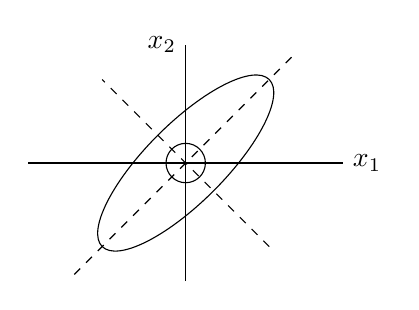
\begin{tikzpicture}
%axis
\draw[](-2,0)--(2,0)node[right]{$x_1$};
\draw[](0,-1.5)--(0,1.5)node[left]{$x_2$};
%
\draw (0,0) circle (0.25);
\draw[rotate=45] (0,0) circle (1.5 and 0.5);
%
\draw[dashed](45:-2)--++(45:4);
\draw[dashed](135:-1.5)--++(135:3);
\end{tikzpicture}
\caption{صدر محور کو نقطہ دار لکیر سے ظاہر کیا گیا ہے۔ (مثال \حوالہ{مثال_آئگنی_جھلی_صدر_محور})}
\label{شکل_مثال_آئگنی_جھلی_صدر_محور}
\end{figure}
\انتہا{مثال}
%=========================
\ابتدا{مثال}\quad امکانی شماریاتی عمل\\
صفحہ \حوالہصفحہ{مثال_خطی_الجبرا_امکانی_شماریاتی_قالب} پر مثال \حوالہ{مثال_خطی_الجبرا_امکانی_شماریاتی_قالب} میں  شہری رقبے کی استعمال کی تقسیم پر غور کیا گیا۔یہ عمل آخر کار  \اصطلاح{تحدیدی حال}\فرہنگ{حال!تحدیدی}\حاشیہب{limit state}\فرہنگ{state!limit} تک پہنچ جائے گا جس کے بعد اس میں مزید تبدیلی رو نما نہیں ہو گی۔یوں امکانی شماریاتی قالب \عددی{\bM{A}\bm{x}=\bM{x}} پر پورا اترے گا۔اس مساوات کی آئگنی قدر اکائی ہے جبکہ آئگنی سمتیہ \عددی{\bM{x}} درکار رقبے کی حتمی تقسیم ہے۔ یوں ہم  \عددی{\bM{A}} سے رو نما ہونے والے عمل کی طویل مدتی اثرات جان سکتے ہیں۔ 

اس مثال میں 
\begin{align*}
\bM{A}=\begin{bmatrix}
0.8&0.1&0\\0.2&0.7&0.1\\0&0.2&0.9
\end{bmatrix}
\end{align*}
ہے جس کے آئگنی اقدار \عددی{\tfrac{7-\sqrt{2}}{10}}، \عددی{\tfrac{7+\sqrt{2}}{10}} اور \عددی{1} ہیں۔ہمیں اکائی آئگنی قدر \عددی{\lambda=1} سے غرض ہے جو \عددی{[1\,\,2\,\,4]^T} ہے۔یوں شہر میں آخر کار رہائشی، تجارتی اور صنعتی تقسیم رقبہ بالترتیب \عددی{1}، \عددی{2} اور \عددی{4} تناسب سے ہو گی۔
\انتہا{مثال}
%=============================
\ابتدا{مثال}\شناخت{مثال_آئگنی_لزلی}\quad نمو آبادی کا \اصطلاح{لزلی نمونہ}\\ 
\اصطلاح{لزلی نمونہ}\فرہنگ{لزلی نمونہ}\حاشیہب{Leslie model}\فرہنگ{Leslie model} جو عمر کے لحاض سے آبادی میں اضافہ بتاتا ہے پر غور کرتے ہیں۔لزلی نمونے میں عمر کے لحاض سے آبادی کی گروہ بندی کی جاتی ہے اور نظر عموماً صرف مادہ جانور پر رکھی جاتی ہے۔فرض کریں کہ کسی جانور کی آبادی میں مادہ جانور کی زیادہ سے زیادہ عمر \عددی{12} سال ہے۔ہم مادہ آبادی کو چار سال کے برابر وقفے سے تین گروہوں میں تقسیم کرتے ہیں۔فرض کریں کہ لزلی قالب درج ذیل ہے۔
\begin{align*}
\bM{L}=[l_{jk}]=\begin{bmatrix} 0& 2.3&0.4\\0.6&0&0\\0&0.3&0 \end{bmatrix}
\end{align*}
لزلی قالب میں  \عددی{l_{1k}} سے مراد \عددی{k} گروہ میں رہتے ہوئے  ایک مادہ سے پیدا ہونے والی بیٹیوں کی اوسط تعداد ہے جبکہ گروہ \عددی{j-1} سے گروہ \عددی{j} تک زندہ پہنچنے والی مادہ کی تناسب کو \عددی{l_{j,j-1}(j=2,3)} سے ظاہر کیا جاتا ہے۔پہلی چار سال کی عمر میں کم عمری کی بنا مادہ بچہ نہیں دیتی لہٰذا \عددی{l_{11}=0} ہے۔اسی طرح پانچ تا آٹھ سال کی عمر میں جوان مادہ زیادہ سے زیادہ (اوسطاً \عددی{2.3}) بچے  دیتی ہے جبکہ ضعیفی  میں مادہ  اوسطاً \عددی{0.4} بچے دیتی ہے۔اسی طرح بچوں کا \عددی{0.6} حصہ یعنی \عددی{\SI{60}{\percent}}  جوانی تک پہنچ پاتا ہے جبکہ جوان جانوروں کا \عددی{0.3} حصہ یعنی \عددی{\SI{30}{\percent}} بڑھاپے تک پہنچتا ہے۔ 

 (الف) اگر ہر گروہ  کی ابتدائی مادہ  آبادی \عددی{2600} ہو تب \عددی{4}، \عددی{8} اور \عددی{12} سال بعد ان گروہوں کی مادہ آبادی کیا ہو گی؟ (ب)  ان گروہوں کی ابتدائی آبادی کیا ہونے سے تمام گروہوں میں تبدیلی کی تناسب برابر ہو گی؟ یہ تناسب کیا ہو گی؟

حل: (الف) ابتدائی طور پر \عددی{\bM{x}_0=[2600\,\,\,\,,2600\,\,\,\,2600]^T} ہے۔چار سال بعد گروہ بندی درج ذیل ہو گی۔
\begin{align*}
\bM{x}_4=\bM{L}\bM{x}_0=\begin{bmatrix} 0& 2.3&0.4\\0.6&0&0\\0&0.3&0 \end{bmatrix}\begin{bmatrix}2600\\2600\\2600  \end{bmatrix}=
\begin{bmatrix}7020\\1560\\780  \end{bmatrix}
\end{align*}
اسی طرح آٹھ سال بعد آبادی \عددی{\bM{x}_8=\bM{L}\bM{x}_4=\bM{L}^2\bM{x}_0=[3900\,\,\,\,4212\,\,\,\,468]^T} اور بارہ سال بعد آبادی
 \عددی{\bM{x}_{12}=\bM{L}\bM{x}_8=\bM{L}^3\bM{x}_0=[9875\,\,\,\, 2340\,\,\,\,1264]^T} ہو گی۔

(ب) متناسب تبدیلی آبادی دریافت کرنے کی خاطر ہمیں ایسا آئگنی سمتیہ \عددی{\bM{x}} درکار ہے جو  \عددی{\bM{L}\bM{x}=\lambda\bM{x}} پر پورا اترتا ہو جہاں \عددی{\lambda>0} آبادی میں اضافے کے تناسب اور \عددی{\lambda<0} آبادی میں کمی کے تناسب کو ظاہر کرے گا۔امتیازی مساوات لکھتے ہیں
\begin{align*}
\begin{vmatrix} -\lambda& 2.3&0.4\\0.6&-\lambda&0\\0&0.3&-\lambda \end{vmatrix}=-\lambda^3+1.38\lambda+0.072=0
\end{align*}
جس کے آئگنی اقدار \عددی{\tfrac{6}{5}}، \عددی{-\tfrac{\sqrt{30}+6}{10}} اور \عددی{\tfrac{\sqrt{30}-6}{10}} ہیں جنہیں کمپیوٹر کی مدد سے حاصل کیا جا سکتا ہے۔مثبت آئگنی قدر \عددی{\lambda=\tfrac{6}{5}=1.2} آبادی میں اضافے کو ظاہر کرتی ہے اور اس کا مطابقتی آئگنی سمتیہ درج ذیل ہے
\begin{align*}
\bM{L}\bM{x}-\lambda \bM{x}=\begin{bmatrix} -1.2&2.3&0.4\\0.6&-1.2&0\\0&0.3&-1.2 \end{bmatrix}\begin{bmatrix}x_1\\x_2\\x_3  \end{bmatrix}=0\quad \implies \quad \bM{x}=\begin{bmatrix} 8\\4\\1 \end{bmatrix}
\end{align*}
جہاں \عددی{x_3=1} چنتے ہوئے \عددی{x_2=4} اور \عددی{x_1=8} حاصل کیا گیا ہے۔ابتدائی کل آبادی \عددی{{3\times 2600=7800}} حاصل کرنے کی خاطر ہم اس آئگنی سمتیہ کو \عددی{\tfrac{7800}{8+4+1}=600} سے ضرب دیتے ہوئے ابتدائی آبادی درج ذیل حاصل کرتے ہیں۔
\begin{align*}
600[8\,\,\,\,4\,\,\,\,1]^T=[4800\,\,\,\,2400\,\,\,\,600]^T
\end{align*}
 آبادی میں تبدیلی کا تناسب \عددی{1.2} فی  چار سال ہو گا۔
\انتہا{مثال}
%===================================

\حصہء{سوالات}
%=============
سوال \حوالہ{سوال_آئگنی_تبدیلی_شکل_الف} تا سوال \حوالہ{سوال_آئگنی_تبدیلی_شکل_ب} میں تبدیلی شکل \عددی{\bM{y}=\bM{A}\bM{x}} کا قالب \عددی{\bM{A}} دیا گیا ہے۔صدر سمتیں اور ان کی مطابقتی سکڑاو یا پھیلاو کا تناسب دریافت کریں۔

%===============
\ابتدا{سوال}\شناخت{سوال_آئگنی_تبدیلی_شکل_الف}\quad
$\begin{bmatrix} 5&2\\2&5 \end{bmatrix}$\\
جوابات:
$3,\, [1\,\,-1]^T, \,\,-45^{\circ};\quad 7,\,[1\,\,1]^T,\,\,45^{\circ}$
\انتہا{سوال}
%===================================
\ابتدا{سوال}\quad
$\begin{bmatrix} 9&8\\8&2 \end{bmatrix}$\\
جوابات:
$-3.23,\, [1\,\,-1.529]^T, \,\,-56.8^{\circ};\quad 14.23,\,[1\,\,0.654]^T,\,\,33.2^{\circ}$
\انتہا{سوال}
%====================================================
\ابتدا{سوال}\quad
$\begin{bmatrix} 1&2\\4&1 \end{bmatrix}$\\
جوابات:
$1-2\sqrt{2},\, [1\,\,-\sqrt{2}]^T, \,\,-54.7^{\circ};\quad 1+2\sqrt{2},\,[1\,\,\sqrt{2}]^T,\,\,54.7^{\circ}$
\انتہا{سوال}
%========================
\ابتدا{سوال}\quad
$\begin{bmatrix} 2&3\\43&12 \end{bmatrix}$\\
جوابات:
$7-\sqrt{34},\, [1\,\,\,\,\tfrac{5-\sqrt{34}}{3}]^T, \,\,-15.5^{\circ};\quad 7+\sqrt{34},\,[1\,\,\,\,\tfrac{5+\sqrt{34}}{3}]^T,\,\,74.5^{\circ}$
\انتہا{سوال}
%=========================
\ابتدا{سوال}\quad
$\begin{bmatrix} 3&1\\5&7 \end{bmatrix}$\\
جوابات:
$2,\, [1\,\,\,\,-1]^T, \,\,-45^{\circ};\quad 8,\,[1\,\,\,\,5]^T,\,\,78.7^{\circ}$
\انتہا{سوال}
%=========================
\ابتدا{سوال}\شناخت{سوال_آئگنی_تبدیلی_شکل_ب}\quad
$\begin{bmatrix} 1.25&0.45\\0.75&2.5 \end{bmatrix}$\\
جوابات:
$1.02,\, [1\,\,\,\,-0.507]^T, \,\,-26.9^{\circ};\quad 2.73,\,[1\,\,\,\,3.285]^T,\,\,73.1^{\circ}$
\انتہا{سوال}
%================================
سوال \حوالہ{سوال_آئگنی_امکانی_شماریاتی_الف} تا سوال \حوالہ{سوال_آئگنی_امکانی_شماریاتی_ب} میں دیے گئے امکانی شماریاتی عمل کا تحدیدی  حال دریافت کریں۔

%===============
\ابتدا{سوال}\شناخت{سوال_آئگنی_امکانی_شماریاتی_الف}\quad
$\begin{bmatrix}0.2&0.5\\0.8&0.5  \end{bmatrix}$\\
جواب:
$\begin{bmatrix}5&8 \end{bmatrix}^T$
\انتہا{سوال}
%===============================
\ابتدا{سوال}\quad
$\begin{bmatrix}0.2&0.5&0.3\\0.3&0.5&0.2 \\0.5&0.2&0.3 \end{bmatrix}$\\
جواب:
$\begin{bmatrix}1&1&1 \end{bmatrix}^T$
\انتہا{سوال}
%===============================
\ابتدا{سوال}\شناخت{سوال_آئگنی_امکانی_شماریاتی_ب}\quad
$\begin{bmatrix}0.4&0.1&0.3\\0.5&0.1&0.2& \\0.1&0.8&0.5 \end{bmatrix}$\\
جواب:
$\begin{bmatrix}29&27&49 \end{bmatrix}^T$
\انتہا{سوال}
%===============================
سوال \حوالہ{سوال_آئگنی_لزلی-الف} اور سوال \حوالہ{سوال_آئگنی_لزلی-ب} میں لزلی نمونے کا قالب \عددی{\bM{L}} دیا گیا ہے (مثال \حوالہ{مثال_آئگنی_لزلی})۔نمو آبادی کا تناسب دریافت کریں۔

%==========
\ابتدا{سوال}\شناخت{سوال_آئگنی_لزلی-الف}\quad
$\begin{bmatrix}0&3.45&0.6\\0.9&0&0\\0&0.45&0 \end{bmatrix}$\\
جواب:\عددی{\tfrac{9}{5}}
\انتہا{سوال}
%==========================
\ابتدا{سوال}\شناخت{سوال_آئگنی_لزلی-ب}\quad
$\begin{bmatrix}0&9&5\\0.4&0&0\\0&0.4&0 \end{bmatrix}$\\
جواب:\عددی{2}
\انتہا{سوال}
%========================
سوال \حوالہ{سوال_آئگنی_لیونٹف_الف} تا سوال \حوالہ{سوال_آئگنی_لیونٹف_ب}  \اصطلاح{لیونٹف  نمونہ}\فرہنگ{لیونٹف نمونہ}\فرہنگ{نمونہ!لیونٹف}\حاشیہب{Leontief model}\فرہنگ{model!Leontief} برائے اخراجات و پیداوار پر مبنی ہیں۔

%===============
\ابتدا{سوال}\شناخت{سوال_آئگنی_لیونٹف_الف}
\اصطلاح{لیونٹف نمونہ}\حاشیہد{روس کے وسیلی وسیلی وچ لیونٹف [1906-1999] نے یہ نمونہ پیش کر کے نوبل انعام حاصل کیا۔} صنعت کی پیداوار اور اس کے اخراجات کا تعلق بیان کرتا ہے۔فرض کریں کہ تین صنعتوں کی پیداوار یہی صنعت استعمال کرتے ہیں اور اس تعلق کو درج ذیل \عددی{3\times 3} \اصطلاح{قالب صرف}\فرہنگ{قالب صرف}\حاشیہب{consumption matrix}\فرہنگ{matrix!consumption}  پیش کرتا ہے
\begin{align*}
\bM{A}=[a_{jk}]=\begin{bmatrix} 0.1&0.5&0\\0.8&0&0.4\\0.1&0.5&0.6 \end{bmatrix}
\end{align*}
جہاں \عددی{a_{jk}} صنعت \عددی{k} کی پیداوار کی وہ تناسب  ہے جو صنعت \عددی{j} خرید کر استعمال کرتی ہے۔ فرض کریں کہ صنعت \عددی{j} کی کل پیداوار کی آمدن \عددی{p_j}  ہے۔ہم چاہتے ہیں کہ ایسی قیمتیں دریافت کریں کہ ہر صنعت کی اخراجات اس صنعت کی آمدی کے برابر ہو۔ اس کو بطور مسئلہ \عددی{\bM{A}\bM{p}=\bM{p}} لکھا جا سکتا ہے جہاں \عددی{\bM{p}=[p_1\,\,\,p_2\,\,\,p_3]^T} ہے۔ایسا \عددی{\bM{p}} دریافت کریں کہ \عددی{p_1}، \عددی{p_2} اور \عددی{p_3} غیر منفی ہوں۔

جواب:
$c[10\quad 18\quad 25]^T$
جہاں \عددی{c} مستقل ہے۔
\انتہا{سوال}
%========================
\ابتدا{سوال}
ثابت کریں کہ سوال \حوالہ{سوال_آئگنی_لیونٹف_الف} کے قالب صرف  کے ہر قطار کے ارکان کا مجموعہ اکائی (\عددی{1}) ہو گا اور اس قالب صرف کا آئگنی قدر بھی اکائی ہو گا۔
\انتہا{سوال}
%==============================
\ابتدا{سوال}\شناخت{سوال_آئگنی_لیونٹف_ب}
آزاد لیونٹف نمونے میں پیداوار کا کچھ حصہ یہی صنعت استعمال کرتے ہیں جبکہ باقی حصہ فروخت کیا جاتا ہے۔یوں \عددی{\bM{A}\bM{x}=\bM{x}} (سوال \حوالہ{سوال_آئگنی_لیونٹف_الف}) کی بجائے،   \عددی{\bM{x}-\bM{A}\bM{x}=\bM{y}} ہو گا جہاں \عددی{\bM{x}} پیداوار ہے جبکہ \عددی{\bM{A}\bM{x}} وہ حصہ ہے جو یہی صنعتیں خود استعمال کرتی ہیں لہٰذا \عددی{\bM{y}} وہ حصہ ہے جس کو فروخت کیا جا سکتا ہے۔

\اصطلاح{قالب مانگ}\فرہنگ{قالب!مانگ}\فرہنگ{مانگ!قالب}\حاشیہب{demand matrix}\فرہنگ{matrix!demand}\فرہنگ{demand!matrix}
 \عددی{\bM{y}=[0.1\,\,\,\,0.3\,\,\,\,0.1]^T} کو پورا کرنے کے لئے قالب پیداوار \عددی{\bM{x}} دریافت کریں جہاں قالب صرف درج ذیل ہے۔
\begin{align*}
\bM{A}=\begin{bmatrix} 0.1&0.4&0.2\\0.5&0&0.1\\0.1&0.4&0.4 \end{bmatrix}
\end{align*}
جواب:
$\bM{x}=(\bM{I}-\bM{A})^{-1}\bM{y}=[0.6747\,\,\,\,0.7128\,\,\,\,0.7543]^T$
\انتہا{سوال}
%=================================
سوال \حوالہ{سوال_آئگنی_عمومی_خصوصیات_الف} تا سوال \حوالہ{سوال_آئگنی_عمومی_خصوصیات_ب} آئگنی قدر مسائل کے عمومی خصوصیات پر مبنی ہیں جنہیں آپ نے ثابت کرنا ہے۔ان مسائل میں فرض کریں کہ \عددی{n\times n} قالب \عددی{\bM{A}} کے آئگنی اقدار \عددی{\lambda_1} تا  \عددی{\lambda_n} ہیں جو غیر منفرد ہو سکتے ہیں۔

%===============
\ابتدا{سوال}\شناخت{سوال_آئگنی_عمومی_خصوصیات_الف}
مرکزی وتر کے ارکان کا مجموعہ اور آئگنی اقدار کا مجموعہ برابر ہیں۔
\انتہا{سوال}
%====================
\ابتدا{سوال}\quad طیفی منتقلی\\
\عددی{\bM{A}-k\bM{I}} کے آئگنی اقدار \عددی{\lambda_1-k} تا  \عددی{\lambda_n-k} ہیں جبکہ اس کے آئگنی سمتیات وہی ہیں جو \عددی{\bM{A}} کے آئگنی سمتیات ہیں۔
\انتہا{سوال}
%=========================
\ابتدا{سوال}\شناخت{سوال_آئگنی_غیر_سمتی_ضرب_طاقت}\quad غیر سمتی مضرب، طاقت\\
غیر سمتی مضرب \عددی{k\bM{A}} کے آئگنی اقدار \عددی{k\lambda_1} تا \عددی{k\lambda_n} ہیں جبکہ \عددی{\bM{A}^m} جہاں \عددی{m=1,2,\cdots} ہے کے آئگنی اقدار \عددی{\lambda_1^m} تا \عددی{\lambda_n^m} ہیں۔دونوں صورتوں میں آئگنی سمتیات وہی ہیں جو \عددی{\bM{A}} کے آئگنی سمتیات ہیں۔
\انتہا{سوال}
%=========================
\ابتدا{سوال}\شناخت{سوال_آئگنی_عمومی_خصوصیات_ب}
کثیر رکنی \عددی{p(\bM{A})=k_m\bM{A}^m+k_{m-1}\bM{A}^{m-1}+\cdots+k_1\bM{A}+k_0\bM{I}} کے آئگنی اقدار درج ذیل ہیں
\begin{align*}
p(\lambda_j)=k_j\lambda_j^m+k_{m-1}\lambda_j^{m-1}+\cdots+k_1\lambda_j+k_0
\end{align*}
جہاں \عددی{j=1,2,\cdots} ہے جبکہ اس کثیر رکنی کے آئگنی سمتیات وہی ہیں کو \عددی{\bM{A}} کے آئگنی سمتیات ہیں۔(سوال \حوالہ{سوال_آئگنی_غیر_سمتی_ضرب_طاقت} کے نتائج استعمال کریں۔)
\انتہا{سوال}
%=================================

\حصہ{تشاکلی، منحرف تشاکلی اور قائمہ الزاویہ قالب}
